\documentclass[9pt, apectratio=43,unicode]{beamer}
\usetheme{Moscow}

\usepackage[utf8]{inputenc}
\usepackage[T2A]{fontenc}
\usepackage[main=russian,english]{babel}

\usepackage{amsmath,amssymb}

\renewcommand{\thefootnote}{\fnsymbol{footnote}}
\hypersetup{pdfauthor={Paul Ostanin}}

%\usepackage{concmath}
%\usepackage{euler}

\usepackage{mathtools}

\graphicspath{ {images/} }

\title[New INM RAS Earth ionosphere F region global dynamical model]{New INM RAS Earth ionosphere F region global dynamical model}
\author[Ostanin P. A.]{Ostanin P. A., Kulyamin D. V., Dymnikov V. P. \\ \smallskip \textit{ostanin.pavel@phystech.edu} \\ \smallskip Moscow Institute of Physics and Technology (MIPT)\\ Institute of Numerical Mathematics of Russian Academy of Sciences (INM RAS)}

\date{ }
\newcommand{\colorhref}[2]{\href{#1}{\textcolor{miptbase!30!black}{#2}}}

\begin{document}

\begin{frame}[plain]
\titlepage
\end{frame}

\def\L{\mathcal{L}}

\section{Formulation of the problem}
\begin{frame}\frametitle{Formulation of the problem; vector equation}
\begin{itemize}
\item[•] Developing the dynamical 3-D Earth ionosphere model (F layer);
\item[•] Providing the coupled numerical ionosphere and thermosphere model, combining with the existing INM RAS thermosphere model.
\end{itemize}

Equation, describing the electron concentration evolution (follows from the continuity equation): $$\dfrac{\partial n_i}{\partial t} = -div(n_i \vec{u}_\parallel)-div\left(n_i\dfrac{1}{B^2}[\vec{E}\times \vec{B}] \right)+$$ $$+div\left(D\left[\nabla_\parallel n_i +n_i\dfrac{1}{T_p}\nabla_\parallel T_p - \dfrac{n_i m_i}{2kT_p}\vec{g}_\parallel\right]\right)+[P-k_in_i].$$

Taken assumptions:
\begin{itemize}
\item[•] The ambipolar diffusion is the dominating dynamic process;
\item[•] Taking into account only the F layer;
\item[•] Plasma is taken quasineutral;
\item[•] The only considered ion is $O^+$;
\item[•] The earth magnetic field is taken dipole;
\item[•] Geographical and magnetic poles are considered to coinside.
\end{itemize}


\end{frame}

\begin{frame}\frametitle{Equation in spherical coordinates in the assumption of a thin spherical layer}

$$\dfrac{\partial n_i}{\partial t} = DYZ(n_i)+DTr(n_i)+[P-kn_i].$$

$$DYZ(n_i) = \dfrac{1}{a\cos\varphi}\dfrac{\partial}{\partial\varphi}\left(D\cos\varphi\left[\dfrac{1}{a}\dfrac{\partial n_i}{\partial\varphi} \cos^2 I -\dfrac{\partial n_i}{\partial z}\cos I\sin I\right]\right)+ \dfrac{\partial}{\partial z}\bigg(D\bigg[\dfrac{\partial n_i}{\partial z}\sin^2 I -$$ $$- +Tr(n_i)+Tr(n_i)\dfrac{1}{a}\dfrac{\partial n_i}{\partial\varphi}\cos I \sin I\bigg]\bigg);$$ 

$$DTr(n_i) = \dfrac{1}{a\cos\varphi}\dfrac{\partial}{\partial \varphi}\bigg[\bigg(\dfrac{1}{a}\dfrac{1}{T_p}\dfrac{\partial T_p}{\partial\varphi}\cos^2 I-\dfrac{1}{T_p}\dfrac{\partial T_p}{\partial z}\cos I \sin I - \dfrac{1}{H}\sin I \cos I\bigg)Dn_i\cos\varphi\bigg] +$$ $$+ \dfrac{\partial}{\partial z}\bigg[\bigg(-\dfrac{1}{a}\dfrac{1}{T_p}\dfrac{\partial T_p}{\partial \varphi}\cos I \sin I +\dfrac{1}{T_p}\dfrac{\partial T_p}{\partial z}\sin^2 I+\dfrac{1}{H}\sin^2I\bigg)Dn_i\bigg].$$
%\end{frame}

%\begin{frame}\frametitle{Upper boundary condition}

At the upper boundary the electron flux is considered to be known and close to zero. In this work it is taken 0. The corresponding upper boundary condidion:
$$D\left(\dfrac{\partial n}{\partial z} \sin^2 I - \dfrac{1}{a}\dfrac{\partial n}{\partial \varphi} \cos I \sin I + \dfrac{1}{H} n \cdot \sin^2 I\right) = F_{ub} \approx 0.$$
\end{frame}


\section{Numerical modelling: two approaches and comparison}

\subsection{Spatial approximation}

\begin{frame}\frametitle{Spatial approximation}
\begin{itemize}
\item[•] For the diffusion components standard conservative approximation with central difference is used:

$$\dfrac{\partial}{\partial z}D\dfrac{\partial n}{\partial z} \approx \dfrac{1}{h_{i+1/2}}\left(\dfrac{D_{i+1/2}(n_{i+1}-n_i)}{h_i}-\dfrac{D_{i-1/2}(n_{i}-n_{i-1})}{h_{i-1}}\right);$$

\item[•] Transfer components are also approximated with central difference formula;


\parbox[b][5cm][t]{50mm}{
\item[•] Key issue and difficulty: existence of mixed derivatives. Second order approximation formula, depending on the sign of $\sin I$ is used.

\item[•] Upper boundary condition is approximated with directed difference, consistent with the main equation approximation.
}
\hfill
\parbox[b][5cm][t]{60mm}{
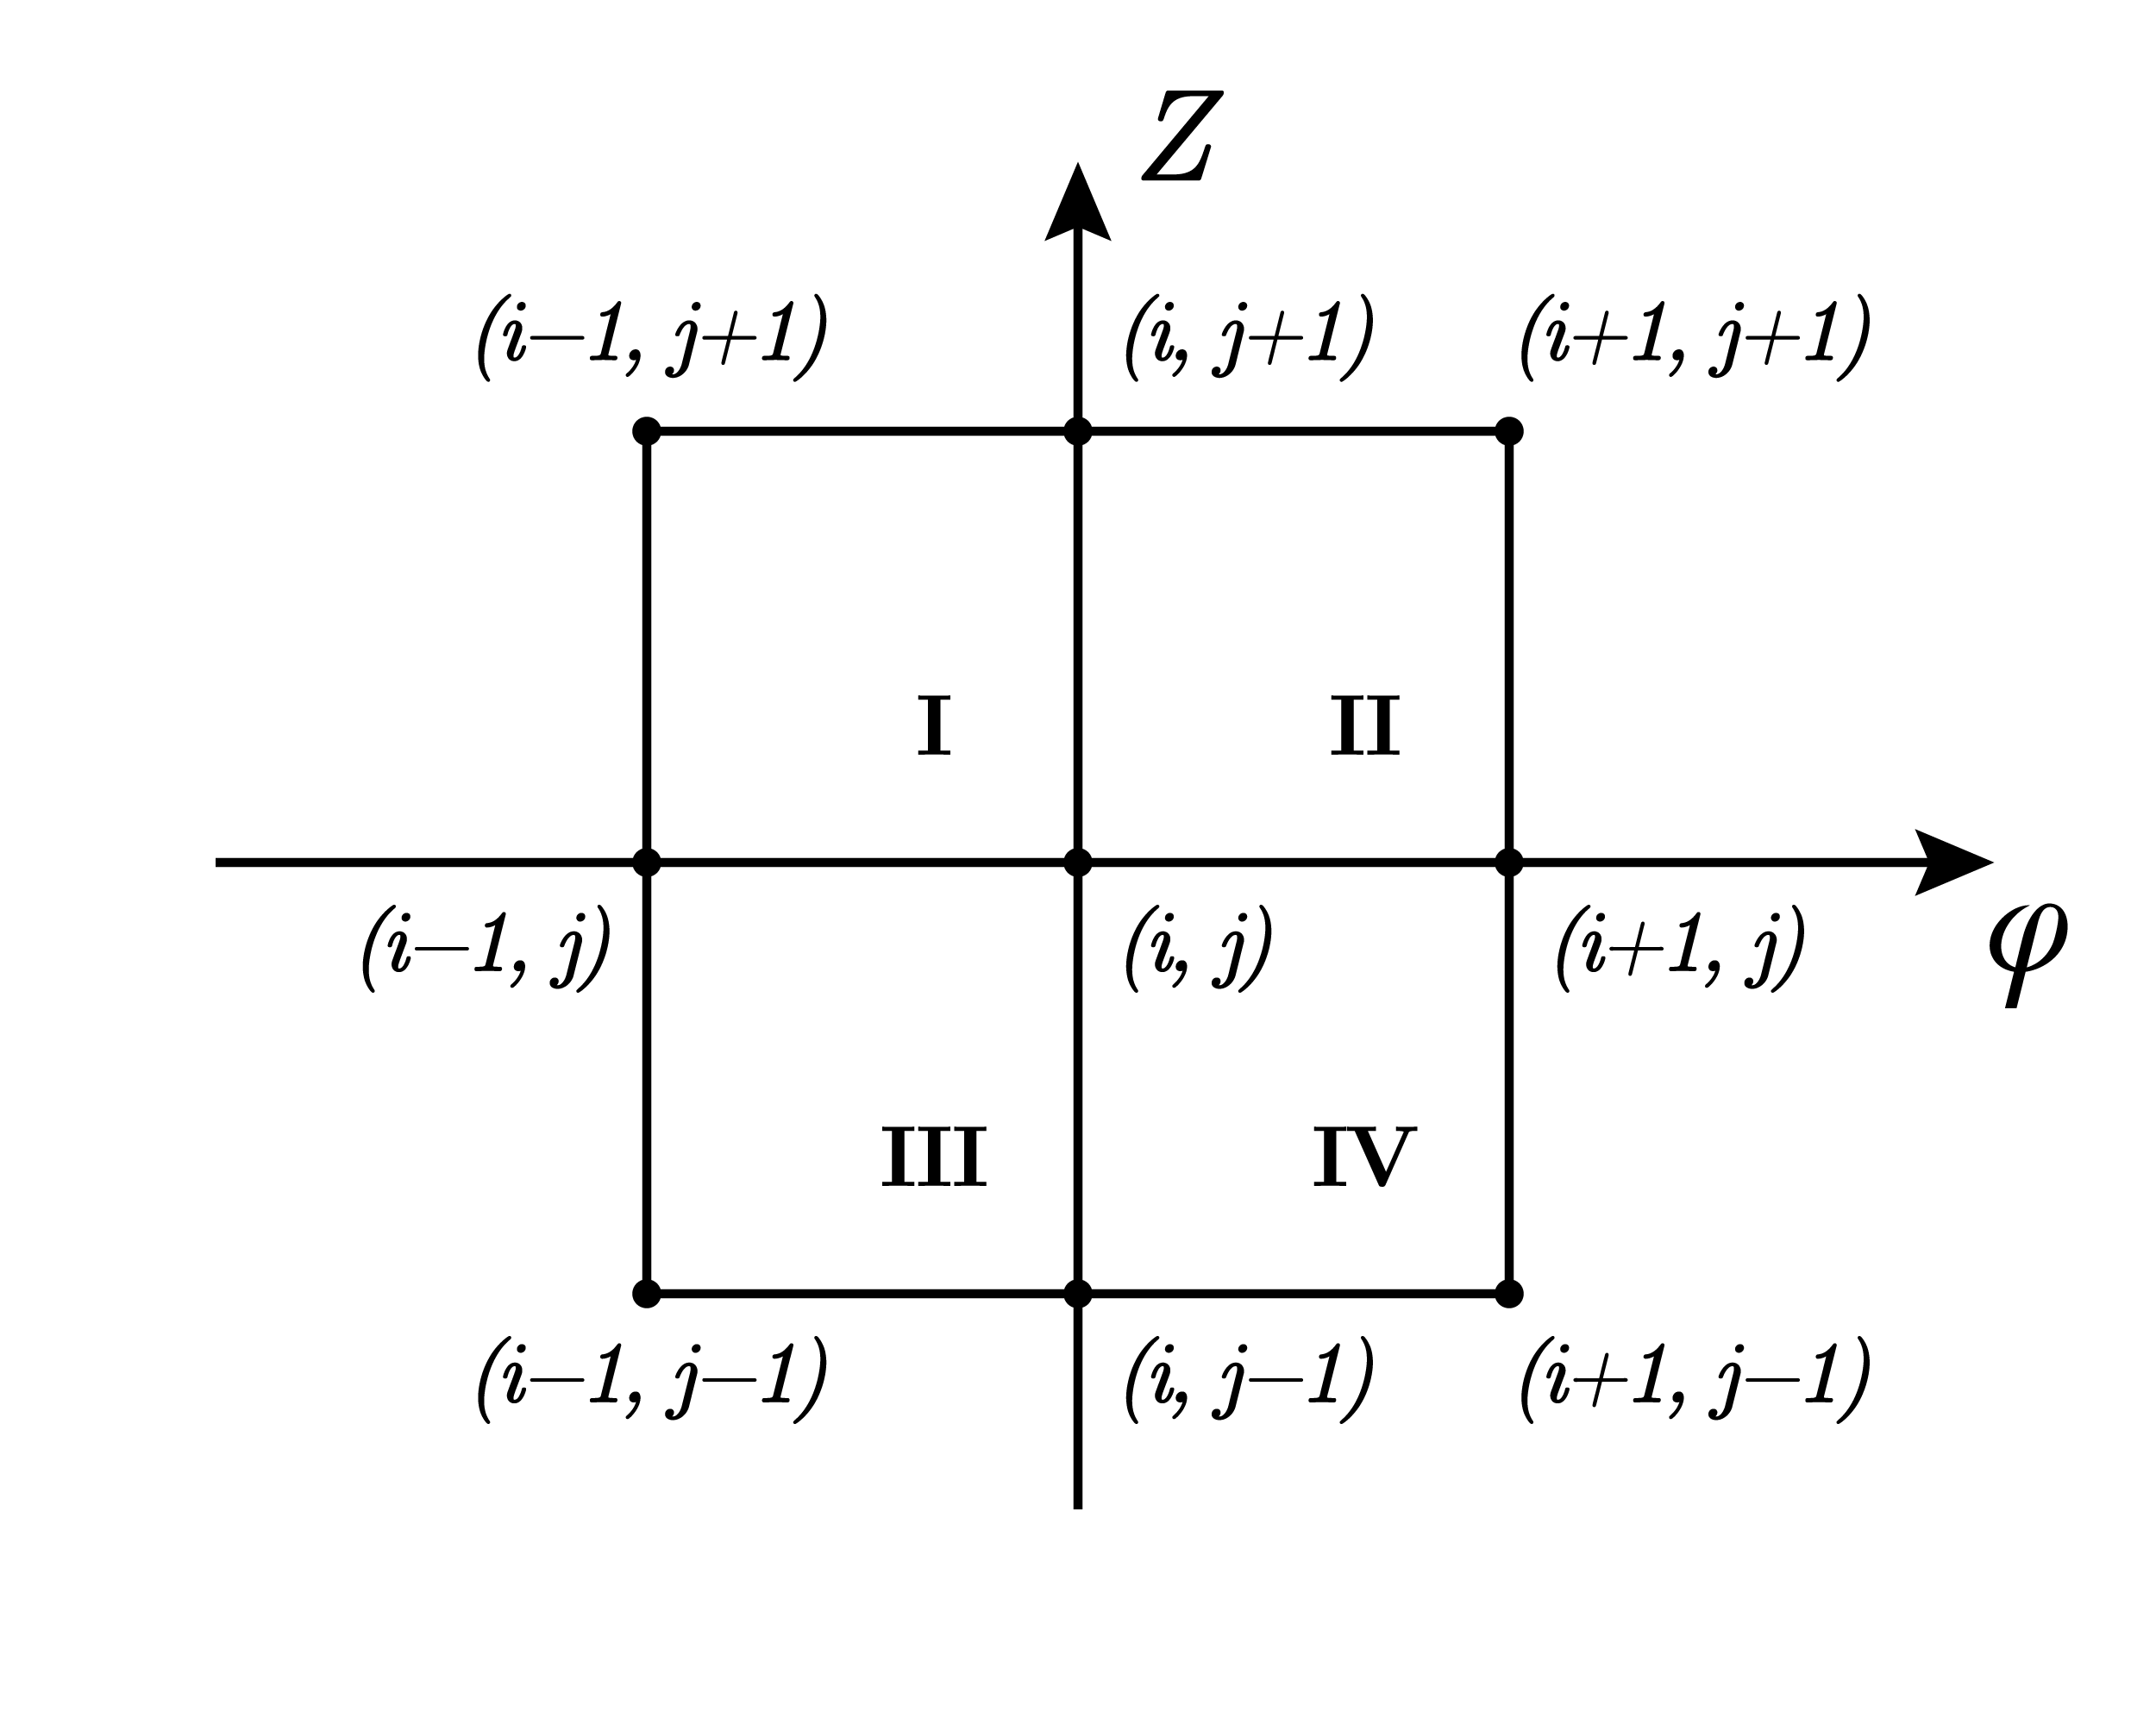
\includegraphics[scale = 0.3]{square}
}

\end{itemize}

\end{frame}


\subsection{Two time approximation methods and model solution}
\begin{frame}\frametitle{Two time approximation methods and model solution}

In this work two different approaches to solving the equation are compared:

\begin{itemize}

\item[I.] 2D implicit scheme: all components of spatial approximation are taken implicitly (linear system is solved with BiCG Stabilized iteration method);

\item[II.] Splitting method: 

\end{itemize}

\begin{itemize}

\item[•] $z$-diffusion, mixed derivatives and photochemistry~---~first splitting step; 

\item[•] diffusion along longitude~---~second splitting step;

\end{itemize} 

(linear system is solved with tridiagonal matrix algorithm);

\bigskip 

\parbox[b][5cm][t]{50mm}{
Scheme properties and convergence nuances are tested on the stationary model solution: $$n_{mod}(z, \varphi) = A\cdot e^{-B(z-C)}\cdot(z-C)\cos^2\dfrac{\varphi}{2}$$ with proper photoionization and upper flux functions $P(z, \varphi)$ and $F_{ub}(\varphi)$.}
\hfill
\parbox[b][5cm][t]{60mm}{
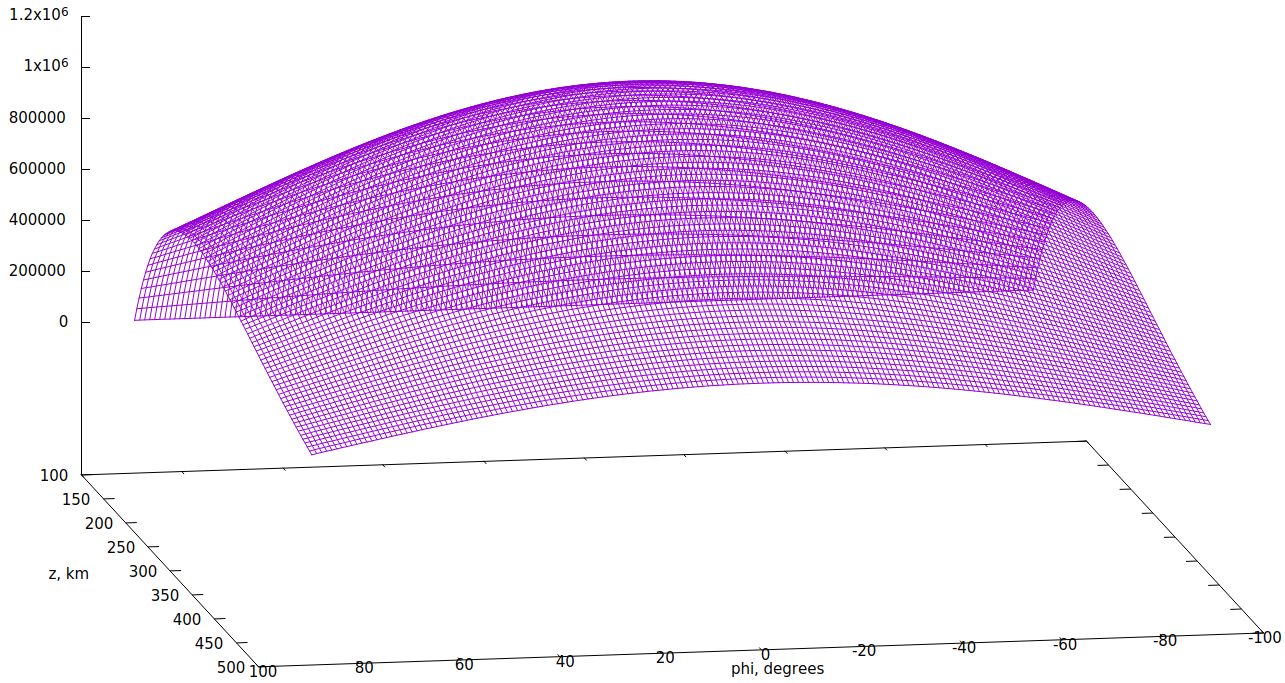
\includegraphics[scale = 0.13]{model}\\Figure 1. Model solution $n_{mod}(z, \varphi)$ from
$100$ km to $500$ km and $\varphi$ from $-90^\circ$ to $90^\circ$.
}
\end{frame}


\subsection{Time approximation comparison}
\begin{frame}\frametitle{Time approximation comparison}

\begin{itemize}

\item[I.] Implicit scheme is significantly more precise;

\item[II.] Splitting method is 4 times faster (with respect to tridiagonal matrix algorithm), but additional time approximation error gives sizeable error;

\end{itemize}

\begin{figure}[H]
\begin{minipage}[c]{0.490\linewidth}
\flushleft
\center{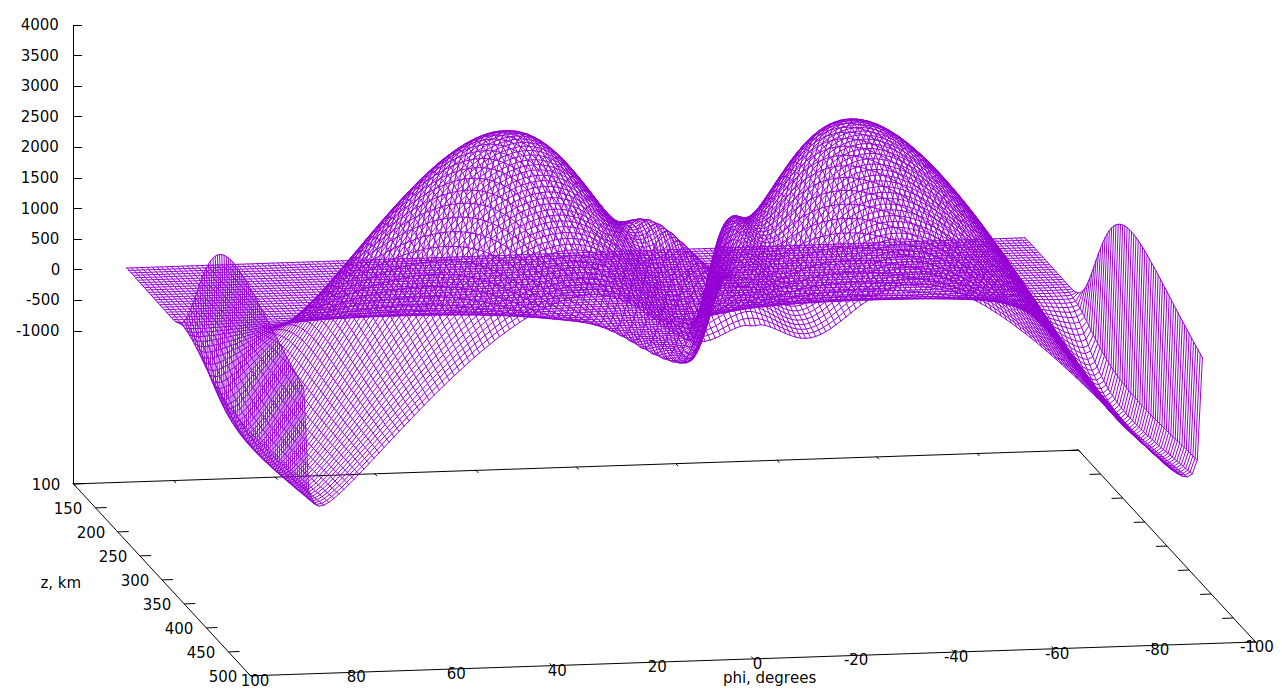
\includegraphics[scale=0.135]{diff_implicit} \\Figure 2. Error in the stationary solution for the implicit method, implemented for model solution.}
\end{minipage}
\hfill
\begin{minipage}[c]{0.490\linewidth}
\flushleft
\center{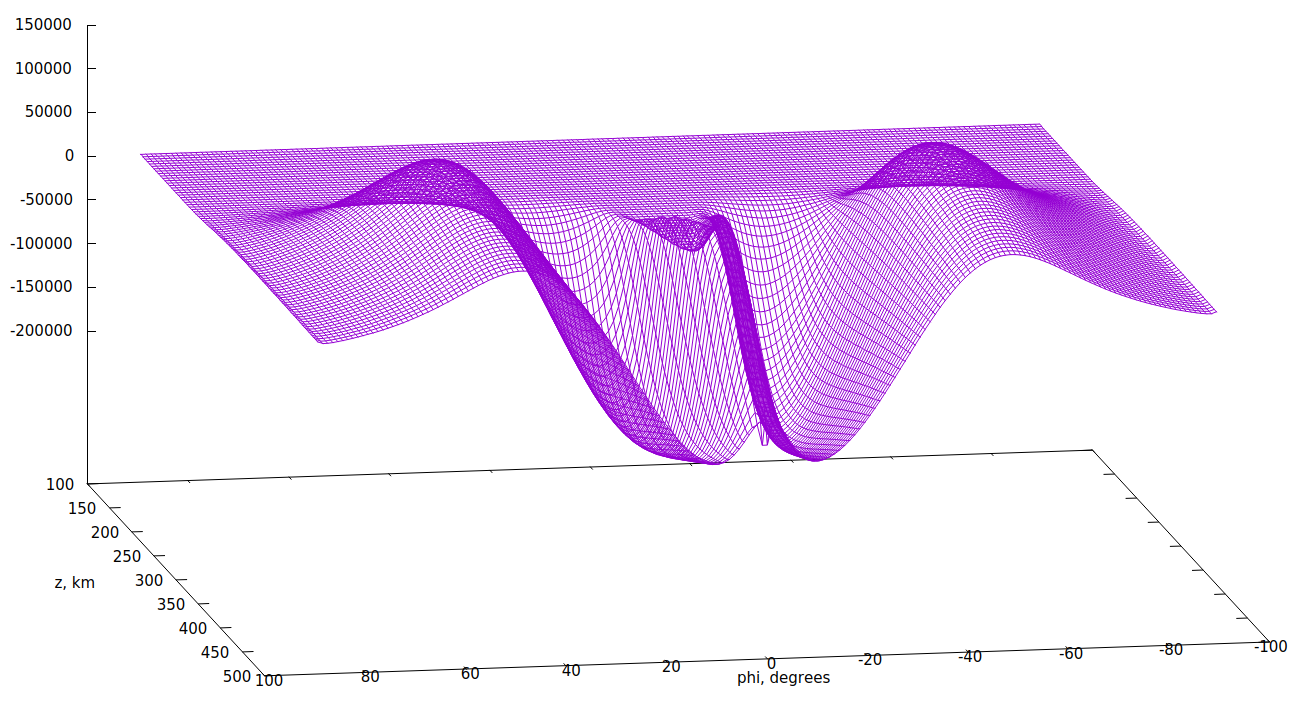
\includegraphics[scale=0.135]{splitted_tau_100}\\Figure 3. Error in the stationary solution for the splitting method, implemented for model solution, with time step  $\tau = 100$.}
\end{minipage}
\end{figure}

The relative error for the splitting method with different time steps is presented in a table below:
\begin{center}
\begin{tabular}{|c|c|c|c|}
\hline
 $\tau$, sec & 100 & 10 & 1\\
\hline
Relative error, $\%$ & $17$ & $4$ & $0{,}5$\\
\hline
\end{tabular}
\end{center}
\end{frame}



\subsection{Daytime stationary solution and diurnal evolution}
\begin{frame}\frametitle{Daytime stationary solution and diurnal evolution}

During the diurnal evolution modelling the photoionization function $P$ is changed in time according the zenith angle $\chi$ evolution: $$P(z, t) = \begin{cases} P_0(z)\cdot e^{\tau_0(z)(1-\sec\chi)}, |\chi|\leq\dfrac{\pi}{2};\\ 0, |\chi|\geq\dfrac{\pi}{2}.\end{cases}$$

\begin{figure}[H]
\begin{minipage}[c]{0.490\linewidth}
\flushleft
\center{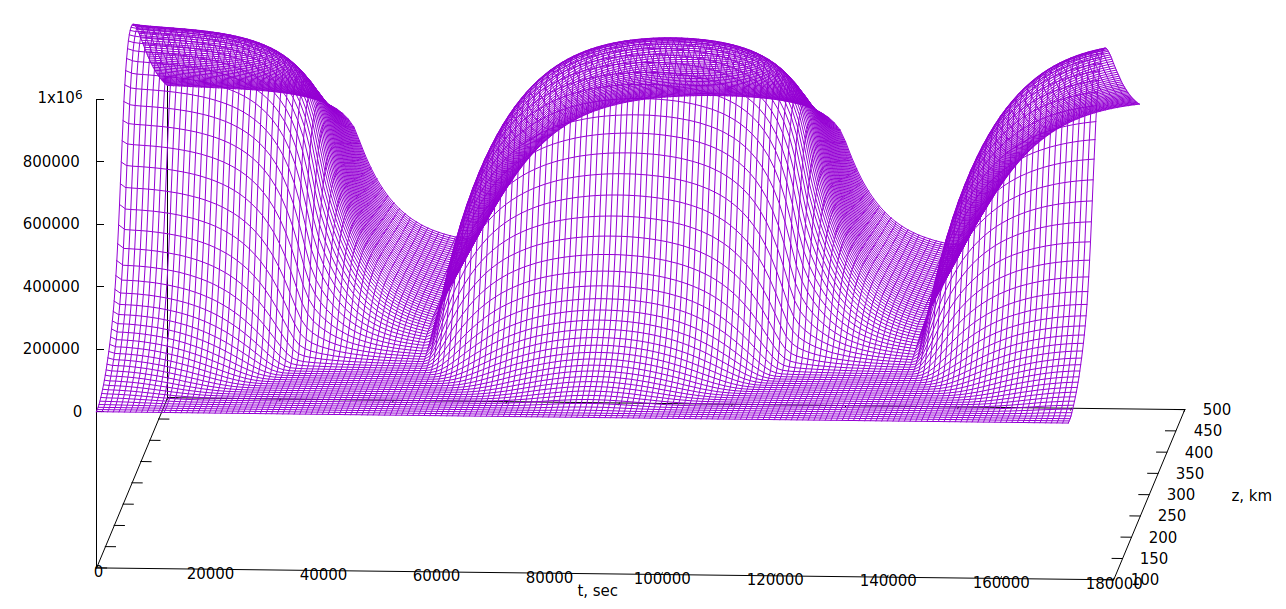
\includegraphics[scale=0.135]{diurnal_implicit}} %\\Figure 2. Error in the stationary solution for the implicit method, implemented for model solution.}
\end{minipage}
\hfill
\begin{minipage}[c]{0.490\linewidth}
\flushleft
\center{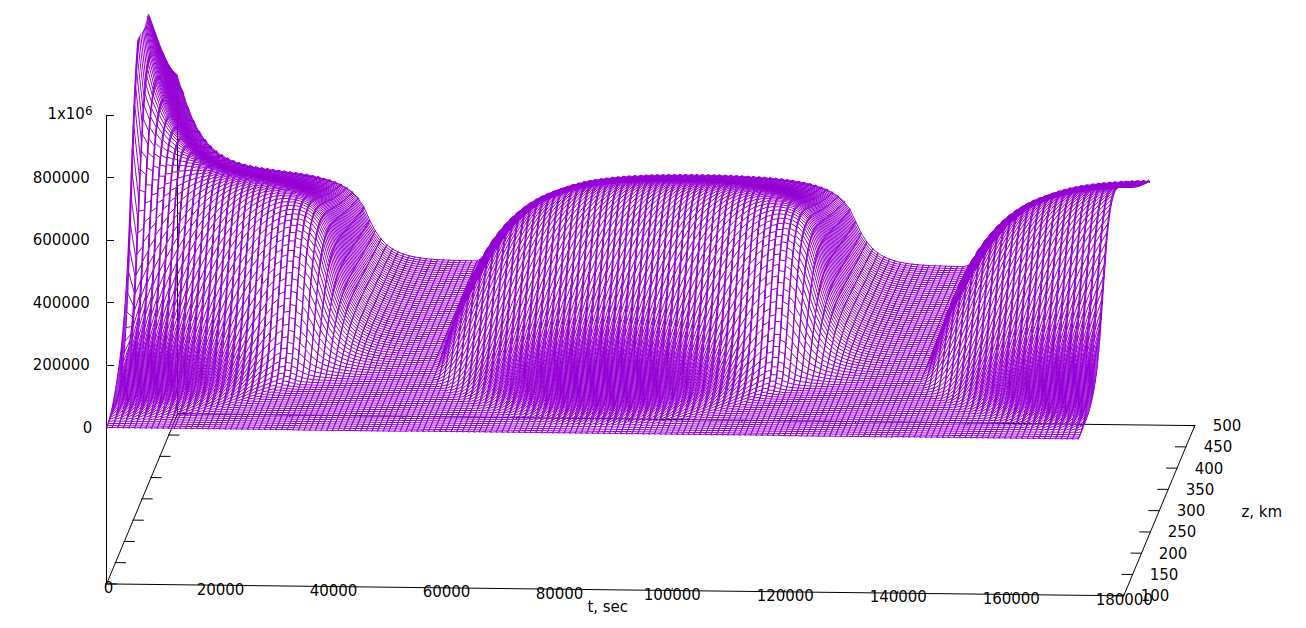
\includegraphics[scale=0.135]{diurnal_splitted}} %\\Figure 3. Error in the stationary solution for the splitting method, implemented for model solution, with time step  $\tau = 100$.}
\end{minipage}

Figure 4. The diurnal evolution of the ion concentration at the latitude $60^\circ$, calculated with the implicit scheme (left) and results obtained from splitted scheme (right).
\end{figure}



\end{frame}



\end{document}
